\documentclass[10pt,a4paper]{report}
\usepackage[utf8]{inputenc}
\usepackage[russian]{babel}
\usepackage[OT1]{fontenc}
\usepackage{amsmath}
\usepackage{amsfonts}
\usepackage{amssymb}
\usepackage{graphicx}
\author{Баратынский А.И.}
\title{Отчет по лабораторной работе на тему: "Визуализация сигналов во временной и частотной области"\newline Дисциплина: "Телекоммуникационные системы и сети"}
\date{13 марта 2014}
\begin{document}
\maketitle
\pagebreak
\chapter{Теоретическая часть}
\section{Цель работы}
Познакомиться со средствами генерации сигналов и визуализации их спектров.
\section{Постановка задачи}
В командном окне MATLAB и в среде Simulink промоделировать чистый синусоидальный сигнал,
также синусоидальный сигнал с шумом. Получить их спектры.
\chapter{Ход работы}
\section{Код MATLAB}
function main()\newline
x=0:0.01:4*pi;\newline
f0 = 5;\newline
\%исходный сигнал\newline
y = sin(2*pi*f0*x);\newline
figure(1)\newline
plot(x(1:200),y(1:200))\newline
grid\newline
\%спектр исходного сигнала\newline
figure(2)\newline
spectrum = fft(y,1024);\newline
normspectrum = spectrum.*conj(spectrum)/1024;\newline
f=100*(0:1023)/1024;\newline
plot(f, normspectrum(1:1024))\newline
axis([0 max(f) 0 10])\newline
grid\newline
\%зашумленный сигнал\newline
ynoize = y+ 0.5*rand(size(x));\newline
figure(3)\newline
plot(x(1:200),ynoize(1:200));\newline
grid\newline
\%спектр зашумленного сигнала\newline
spectrum = fft(ynoize,1024);\newline
noizespectrum = spectrum.*conj(spectrum)/1024;\newline
figure(4)\newline
plot(f, noizespectrum())\newline
axis([0 max(f) 0 10])\newline
grid\newline
\section{Результаты работы}
Графики временной и частотной характеристик исходного и зашумленного синусоидальных сигналов:
\begin{figure}
\begin{center}
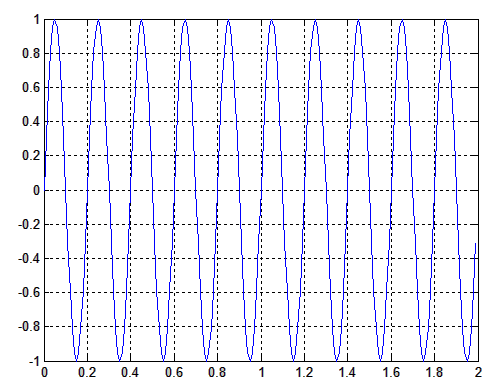
\includegraphics[angle=0, scale = 1]{pic1.png}\newline
Рис. 1 Исходный сигнал\newline
\end{center}
\begin{center}
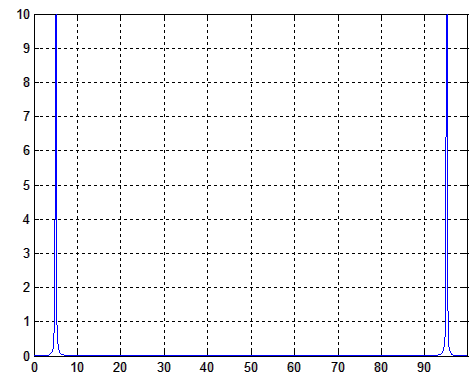
\includegraphics[angle=0, scale = 1]{pic2.png}\newline
Рис. 2. Спектр исходного сигнала\newline
\end{center}
\end{figure}
\begin{figure}
\begin{center}
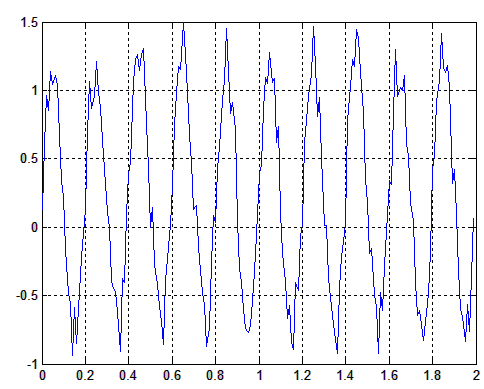
\includegraphics[angle=0, scale = 1]{pic3.png}\newline
Рис. 3. Зашумленный сигнал\newline
\end{center}
\begin{center}
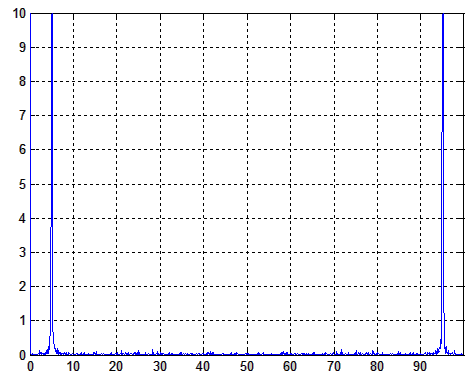
\includegraphics[angle=0, scale = 1]{pic4.png}\newline
Рис. 4. Спектр зашумленного сигнала\newline
\end{center}
\end{figure}
\chapter{Вывод}
В данной лабораторной работе были получены исходный сигнал(синус), его спектр, зашумленный сигнал и спектр зашумленного сигнала. 
\end{document}